\documentclass[12pt, letterpaper]{article}
\usepackage{graphicx} % Required for inserting images
\graphicspath{{./figures/}}
\usepackage{listings} % Required for inserting code
\lstset{inputpath=./src/}
\usepackage{xcolor} % Required for formatting code

\title{Assignment 2 - LaTeX Write Up}
\author{Connor Fleischman}
\date{November 1, 2024}

\definecolor{background}{rgb}{0.95,0.95,0.92}
\definecolor{codegreen}{rgb}{0,0.6,0}
\definecolor{codegray}{rgb}{0.5,0.5,0.5}
\definecolor{codepurple}{rgb}{0.58,0,0.82}
\definecolor{magenta}{rgb}{1,0,1}
\definecolor{backcolour}{rgb}{0.95,0.95,0.92}
\definecolor{keywordcolor}{rgb}{0.82,0.1,0.26}

\lstdefinestyle{mystyle}{
   backgroundcolor=\color{background},   
   commentstyle=\color{codegreen},
   keywordstyle=\color{keywordcolor}\bfseries,
   numberstyle=\tiny\color{codegray},
   stringstyle=\color{codepurple},
   basicstyle=\ttfamily\small,
   frame=single, 
   rulecolor=\color{codegray},
   breakatwhitespace=false,         
   breaklines=true,                 
   captionpos=b,                    
   keepspaces=true,                 
   numbers=left,                    
   numbersep=10pt, 
   showspaces=false,                
   showstringspaces=false,
   showtabs=false,                  
   tabsize=4,
   emph={int,char,double,float,unsigned}, 
   emphstyle={\color{blue}},
}

\lstset{style=mystyle}

\begin{document}
\maketitle
\begin{center}
   
\includegraphics[width=120mm,scale=0.5]{MaristSeal.png}
\end{center}
\newpage

%%%%%%%%%%%%%%%%%%%%%%%%%%%%%%%%%%%%%%%%%%%%%%%%%%%%%%%%%%%%%%%%%%%%%%%%%%%%%%%%%%%%%%%%%%%%%%%%%%%
\section{Assignment Results}
Assignment 02 was to perform different searches on the magic items text file provided in Assignment 01 for 42 random keys, picked from magic items.

\subsection{Linear Search} \label{LinSch}
The first search to be performed was a linear search.
This searching method takes a key and sequentially picks through each magic item, comparing the current item to the key, until the key is found.
After implementing this in C++ and ensuring that my algorithm is correct, 10 tests were performed and their data recorded below.
\begin{center}
   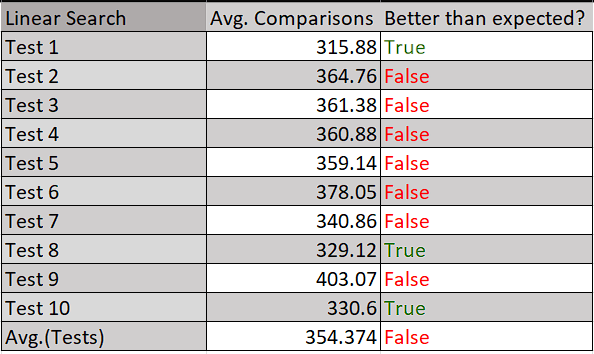
\includegraphics[width=120mm,scale=0.5]{LinSearch.png}
\end{center}
This table diagrams the average time each test took to find all 42 keys in magic items. 
It also depicts how efficient the algorithm was.
Before we continue, it is important clarify a few prerequisites.
\begin{center}
   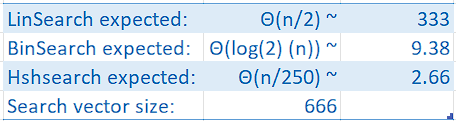
\includegraphics[width=120mm,scale=0.5]{Prerequisites.png}
\end{center}
With these in mind, the "Better than expected?" column now has a basis to compare to.
So over the performed tests, the data shows that only 30\% of all searches for the 42 keys performed were more efficient than the expected value.
Not an amazing look for my code, however only 10 tests were performed, who's to say that if 100 tests took place it wouldn't spread to 50\%?

\subsection{Binary Search} \label{BinSch}
A binary search was the next task to conquer.
This search takes a key and the middle value of the sorted magic items.
Compares if the middle item is or is not the key, if it is not, then it compares if the middle item is larger or smaller than the key.
Finally if the key is larger than the middle item, the search is ran again on the half greater than the middle.
Otherwise the key is smaller and the search is ran on the half smaller than the key.
\begin{center}
   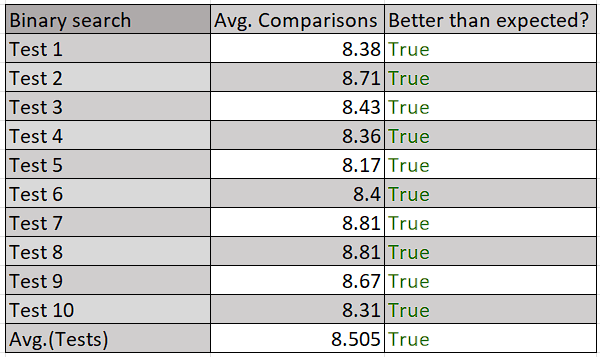
\includegraphics[width=120mm,scale=0.5]{BinSearch.png}
\end{center}
The same 10 tests were performed for binary search with each test's keys being the same for each numbered test.
Meaning, the keys used for test one in linear search were the same keys used for binary search (and for hash searching).
\newline
\indent As shown above, the binary searching algorithm I implemented was quite efficient.
But the same logic applied to linear search applies here, although 100\% of tests were more efficient than the average case, does not mean that with more testing it can't be inefficient.

\subsection{Hash Table Search} \label{HshTblSch}
The last search assigned was to take the magic items, create a hash table of 250 buckets, populate it with the items, and search for the keys using the hash table.
A hash table is a 2-dimensional table where each value in the table has its own table of values.
\newline
\indent So in relation to the problem, the hash table stores each magic item in a bucket corresponding to its ASCII value.
This allows a search to narrow down the possible answers much more quickly than linear and binary search, leading to a much more efficient algorithm.
\begin{center}
   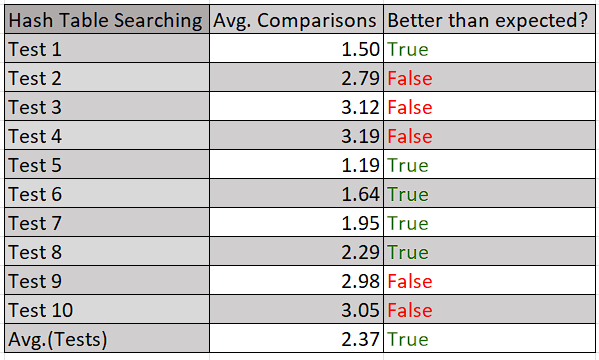
\includegraphics[width=120mm,scale=0.5]{HshSearch.png}
\end{center}
After conducting the same 10 tests, using the same 42 keys per tests, the data has shown that 50\% of tests performed were above the average efficiency of a hash search.
It also shows how efficient hash searching is compared to the other searching algorithms above.
It would be interesting to see if the average of all tests would fall below the expected threshold if more tests were performed.
\newpage

%%%%%%%%%%%%%%%%%%%%%%%%%%%%%%%%%%%%%%%%%%%%%%%%%%%%%%%%%%%%%%%%%%%%%%%%%%%%%%%%%%%%%%%%%%%%%%%%%%%
\section{Code Breakdown - Linear \& Binary Search}
My code consists of three C++ documents. 
A 'main.cpp' file housing the majority of the computations, and two assistive files, 'sortItems.h' and 'buildHashTable.h'.
These files are woven together through 'main.cpp' so that when executed it prints out the results of the searches to the console.
These files are in the './Assignment2/src' folder.

\subsection{Breakdown - main()} \label{Main}
Our program begins through the main function below.
Do not worry if this seems complex, we will break it down piece by piece.
\lstinputlisting[language=C++, firstline=104, lastline=135]{main.cpp}
When the executable is ran a vector of strings called keys is declared and instantiated as sort.first().
This comes from the 'sortItems.h' file which returns a pair, for more detail see section \ref{SrtItm}.
Then sorted is instantiated as sort.second(), from 'sortItems.h', for more detail see section \ref{SrtItm}.
\newline
\indent A linear search is then performed for each key in keys using the sorted magic items.
After, the average comparisons is calculated and produced for that search on each key.
Next a binary search is used for the same keys as before to search through magic items.
Again, the program calculates and produces the average number of comparisons for a key based off the 42 keys.
\newline
\indent Finally, the code clears the sorted list and creates a hash table from 'buildHashTable.h' using createTable().
The same search is performed for the same 42 keys as prior, but instead of searching through the magic items, the program uses a hash table populated with the magic items.
Then the average comparisons is found and output and the comparison count is reset to 0 and keys and the hash table are all cleared.

\subsection{Breakdown - sortItems.h} \label{SrtItm}
The main function firstly uses a function from 'sortItems.h'.
Specifically, it uses the pair of return values given from the sort() method in 'sortItems.h'.
It sets a vector of strings called keys to sort().first, and sorted, which was defined in section \ref{Prereq}, as sort().second afterwards.
\lstinputlisting[language=C++, firstline=13, lastline=48]{sortItems.h}
As we can see on line 35, sort().first is keys and sort().second is the insertionSort() function.
Keys is defined as a vector of strings which, after randomly selecting a starting value within the bounds of the data, we store the next 42 values as keys.
This is done on lines 27-33.
\newline
\indent Insertion sort is defined on line 1 and has a return value of a vector of strings.
Insertion sort takes the unsorted magic items, written to a vector of strings, sorts it using an insertion sort, and returns it to sort().second.
This is why we set 'keys = sort().first' (ln 3, sec \ref{Main}) and 'sorted = sort().second' (ln 4, sec \ref{Main}).
Finally in the sort() function we read the file 'magicItems.txt' into a vector of strings called lines for manipulation.

\subsection{Breakdown - linearSearch()} \label{LinSchCde}
\lstinputlisting[language=C++, firstline=21, lastline=40]{main.cpp}

\subsection{Breakdown - binarySearch()} \label{BinSchCde}
\lstinputlisting[language=C++, firstline=42, lastline=72]{main.cpp}
\newpage

%%%%%%%%%%%%%%%%%%%%%%%%%%%%%%%%%%%%%%%%%%%%%%%%%%%%%%%%%%%%%%%%%%%%%%%%%%%%%%%%%%%%%%%%%%%%%%%%%%%
\section{Code Breakdown - Hash Table Searching}
\subsection{buildHashTable.h} \label{BldHshTbl}
\lstinputlisting[language=C++, firstline=10, lastline=49]{buildHashTable.h}

\subsection{searchItem()} \label{HshSchCde}
\lstinputlisting[language=C++, firstline=83, lastline=102]{main.cpp}
\newpage

%%%%%%%%%%%%%%%%%%%%%%%%%%%%%%%%%%%%%%%%%%%%%%%%%%%%%%%%%%%%%%%%%%%%%%%%%%%%%%%%%%%%%%%%%%%%%%%%%%%
\section{Code Breakdown - Misc.} \label{Misc}
\subsection{averageComparisons()} \label{AvgComp}
Here we are calculating the average number of comparisons needed to find every key in the sorted, or hashed, data set.
\lstinputlisting[language=C++, firstline=74, lastline=81]{main.cpp}
To do to two decimal places, as specified in the Assignment 02 instructions, we must use a fixed precision floating point number.
To find the average of the comparisons we use a globally scoped variable called comparisonCount defined in section \ref{Prereq}.
With this we divide it by the total number of keys, defined in section \ref{SrtItm} on line 3.
This gives us the average which is then output to the console to two decimal places.
Then the comparison count is reset to 0 for the next search.

\subsection{main.cpp - Prerequisites} \label{Prereq}
\lstinputlisting[language=C++, firstline=10, lastline=19]{main.cpp}
Beginning 'main.cpp' we include 'buildHashTable.h' and 'sortItems.h' as well as 'iostream' and 'iomanip'.
These allow us to use functions like createTable() and sort.first() or .second() for our algorithms.
They also allow for use of console output and floating point number precision respectively. 
We also use the std namespace as to not have to add "std::\_" to the code.
\newline
\newline
Globally scoped variables:
\newline
\indent comparisonCount - the total number of comparisons for a search
\newline
\indent sorted - a vector of strings to store the sorted magic items
\newline
\indent hashTable - a vector of vectors of strings, or a vector of buckets of strings

\subsection{sortItems.h - Prerequisites} \label{SrtItmGV}
\lstinputlisting[language=C++, firstline=1, lastline=11]{sortItems.h}

\subsection{buildHashTable.h - Prerequisites} \label{BldHshTblGV}
\lstinputlisting[language=C++, firstline=1, lastline=8]{buildHashTable.h}
\newpage

%%%%%%%%%%%%%%%%%%%%%%%%%%%%%%%%%%%%%%%%%%%%%%%%%%%%%%%%%%%%%%%%%%%%%%%%%%%%%%%%%%%%%%%%%%%%%%%%%%%
\section{Final Thoughts}
% BREAK DOWN CODE DOC BY DOC FUNC BY FUNC, DON'T WORD FOR WORD, INSTEAD SAY WHAT IT DOES, HOW, WHY, EFFICIENCY...
Note the asymptotic running time of each search and explain why it is that way. 
Including the asymptotic running time of	hashing	with chaining and explain why it is that way.
\end{document}